\chapter{Il livello della Macchina Assembler}

\section{Modello a programma memorizzato}

Come già introdotto, il modello di calcolatore adottato comunemente è quello di \textit{Von Neumann} o a programma memorizzato, caratterizzato dal fatto che il linguaggio assembler è di tipo imperativo, quindi facente uso

\begin{enumerate}
    \item del concetto di variabile, e della tecnica di assegnamento e riassegnamento di variabili,
    \item del concetto di sequenzializzazione esplicita delle istruzioni, implementato da una particolare variabile detta contatore di istruzioni, IC (instruction counter).
\end{enumerate}

\noindent Ogni istruzione assembler è rappresentata in binario secondo un certo formato dell'istruzione.\
Tipicamente, il formato dell'istruzione contiene elementi come:

\begin{itemize}
    \item codice operativo dell'istruzione,
    \item informazioni per ricavare indirizzi di variabili o di altre istruzioni,
    \item eventuali costanti,
    \item eventuali opzioni legate all'ottimizzazione del programma e dell'architettura.
\end{itemize}

\noindent Al momento della loro utilizzazione durante l'esecuzione del programma, le variabili possono risiedere in:

\begin{itemize}
    \item  locazioni di memoria principale,
    \item  registri generali.
\end{itemize}

\noindent Il linguaggio assembler deve prevedere un insieme di regole per indirizzare una locazione da parte di un'istruzione:\ tali regole saranno dette \textbf{modi di indirizzamento}.

I registri generali rappresentano, in un certo senso, un'estensione della memoria disponibile al programma.\
Essendo implementati, a livello firmware, nella Parte Operativa del processore, essi sono caratterizzati da un tempo di accesso molto basso, di diversi ordini di grandezza inferiore a quello necessario per leggere o scrivere parole residenti in memoria principale.\
Normalmente, i registri generali sono organizzati in una (piccola) memoria di registri; la sua capacità può variare da poche unità a qualche decina fino alle centinaia (noi supporremo che sia di 64 unità).

Il significato dell'aggettivo ``\textit{generali}'' sta a indicare che l'utilizzo di tali registri non è specifico di una certa funzionalità.\
Un registro generale verrà usato per contenere il valore di una variabile riferita dal programma, ma anche un indirizzo di memoria o una quantità che viene utilizzata per calcolare un indirizzo di memoria, o altre eventuali informazioni manipolabili a livello assembler.

I registri generali sono, ovviamente, visibili anche a livello firmware secondo la specifica struttura che
assumono nella Parte Operativa del processore.

In alcune macchine, il contatore istruzioni è, come i registri generali, \textit{visibile a livello assembler} e su esso sono possibili tutte le operazioni consentite sui registri generali.\
In altre macchine, \textit{IC è visibile solo a livello firmware}, nel senso che la sua manipolazione (modifica) è effettuata dal microprogramma del processore nell'interpretare ogni istruzione assembler.\
In questo secondo caso, esistono comunque istruzioni assembler (\textit{istruzioni di salto}) il cui effetto finale è di modificare il contenuto di IC per fargli assumere un valore fuori sequenza, pur se IC non è riferito esplicitamente dall'istruzione; allo stesso modo, tutte le istruzioni non di salto modificano IC nel senso di incrementarlo per puntare all'istruzione immediatamente successiva in sequenza, ma, a maggior ragione, questo effetto è implicito e IC non è riferito esplicitamente dall'istruzione.

In ogni caso, \textit{la semantica di un'istruzione} deve contenere sempre la manipolazione di IC; si ricorda infatti che la semantica di un comando deve fornire tutti gli elementi che permettano di definirne il supporto (interprete).

\section{Compilazione ed esecuzione}

\subsection{Programmi e processi}

I \textit{moduli di elaborazione} a livello delle applicazioni e a livello del sistemo operativo sono i \textit{processi}:\ programmi sequenziali con propria capacità di controllo, eseguibili con concorrentemente ad altri e cooperanti con essi.

Un qualunque programma \textit{viene compilato in un processo} o, nel caso che il programma stesso sia parallelo, in una collezione di processi.

La fase di linking ha il compito di collegare a ogni processo applicativo i \textit{servizi} di sistema necessari all'esecuzione del programma corrispondente e non visibili esplicitamente nel codice sorgente e di arricchire il processo con un insieme di \textit{informazioni di utilità}, cioè informazioni che sono essenziali per l'esecuzione e la gestione del processo, che sono contenute in una \textit{struttura dati} che chiameremo \textbf{descrittore di processo} (PCB, \textit{Process Control Back}).\
Il PCB stesso fa parte delle informazioni di un processo.

\subsection{Compilazione e caricamento}

La compilazione di un programma è effettuata da un compilatore, il quale, prendendo in ingresso il programma sorgente, lo trasforma in un processo \textit{rappresentato da un \textbf{file oggetto} binario}, o \textbf{codice eseguibile}, contenete tutte le informazioni necessarie per l'esecuzione del processo stesso.

Il procedimento di compilazione costa, operativamente, di più fasi:

\begin{itemize}
    \item traduzione da linguaggio sergente in assembler simbolico;
    \item traduzione da assembler simbolico a codice binario;
    \item linking.
\end{itemize}

\noindent In base alle regole di compilazione legate alla struttura del linguaggio sorgente, il compilatore provvede a generare una lista di istruzioni assembler.\
Nel far questo, un importante compito del compilatore è quello:

\begin{itemize}
    \item dell'allocazione statica della memoria virtuale e dei registri generali,
    \item dell'inizializzazione di una parte delle locazioni di memoria virtuale e registri generali.
\end{itemize}

\noindent Gli indirizzi generati dal processore, durante l'esecuzione di un processo, non sono direttamente indirizzi di memoria principale (\textit{indirizzi fisici}), bensì \textbf{indirizzi logici}, cioè indirizzi riferiti a un'\textit{astrazione} della memoria del processo, detta \textbf{memoria virtuale}.\
Questa può essere vista come un array unidimensionale, con indici (indirizzi logici) a partire da zero fino al massimo necessario per rappresentare il programma o fino al massimo consentito dall'ampiezza dell'indirizzo logico in bit; per una macchina a 32 bit e con indirizzamento alla parola, la massima ampiezza della memoria virtuale di ogni programma è 4G parole.

L'insieme degli indirizzi logici di un processo è detto il suo \textbf{spazio logico di indirizzamento}.

Il codice eseguibile del processo, generato dal compilatore, è quindi riferito alla memoria virtuale.\
Il processore genera indirizzi logici sia per le istruzioni sia per i dati.

Quando un processo viene allocato (o riallocato) in memoria principale, viene stabilita una corrispondenza tra gli indirizzi logici della parte allocata e gli indirizzi fisici in cui viene allocata.\
Questa funzione, detta \textit{funzione di rilocazione} o \textit{di traduzione dell'indirizzo}, è di norma implementata come una tabella associata al processo (\textbf{Tabella di Rilocazione}).

La funzione di rilocazione viene aggiornata ogni volta che l'allocazione del processo viene modificata.

La traduzione dell'indirizzo deve essere effettuata in modo molto efficiente e quindi l'accesso alla Tabelle di Rilocazione viene effettuata con opportune soluzioni hardware-firmware delegate a un'unità interposta tra il Processore e la memoria principale (\textit{Memory Management Unit}, o \textit{MMU}).

\newpage

\section{D-RISC:\ un assembler didattico di tipo Risc}

Le principali caratteristiche della macchina assembler, che chiameremo D-RISC, sono le seguenti:

\begin{itemize}
    \item sono presenti 64 \textit{registri generali} RG[0..63], mentre il registro \textit{contatore istruzioni} (IC) è visibile solo a livello firmware; solo alcune istruzioni, tipicamente di salto o speciali, hanno effetto sul contenuto di IC, ma, a livello assembler, non esiste alcun altro modo di modificare tale registro;
    \item \textit{la parola è di} 32 \textit{bit}:\ questa caratteristica non è comunque vincolante per quanto riguarda la rappresentazione dei dati, che possono essere a 64 bit senza alterare le altre caratteristiche della macchina.\ Come detto sotto, vincolante è invece la lunghezza dell'istruzione e la lunghezza dell'indirizzo logico;
    \item la memoria, sia virtuale sia fisica, è \textit{indirizzabile} alla parola;
    \item \textit{lo spazio di indirizzamento logico di un processo è unidimensionale} e gli indirizzi logici sono di 32 bit.\ Lo spazio di indirizzamento logico di un processo è dunque più ampio al più 4G parole;
    \item le istruzioni sono tutte rappresentate su 32 bit.\ Supporremo che il \textit{codice operativo} sia codificato negli 8 bit più significativi; sono dunque disponibili fino a 256 istruzioni, anche se di fatto ne potranno essere implementate meno.
\end{itemize}

\section{Regole di compilazione e composizione}

\subsection{Comandi condizionali e iterativi}

Indicheremo con \textit{C} un predicato (guardia) e con \textit{B} un comando o blocco (sequenza) di comandi.\ Con IF\_\textit{C} ETICHETTA e IF\_N\_\textit{C} ETICHETTA indicheremo, in generale, le istruzioni assembler di salto condizionato \textit{C} e not \textit{C} rispettivamente.

La compilazione di un comando/blocco \textit{B} nella corrispondente sequenza di istruzioni sarà indicata con \textit{compile} (\textit{B}).

Abbiamo allora le seguenti regole:

\begin{figure}[H]
    \centering
    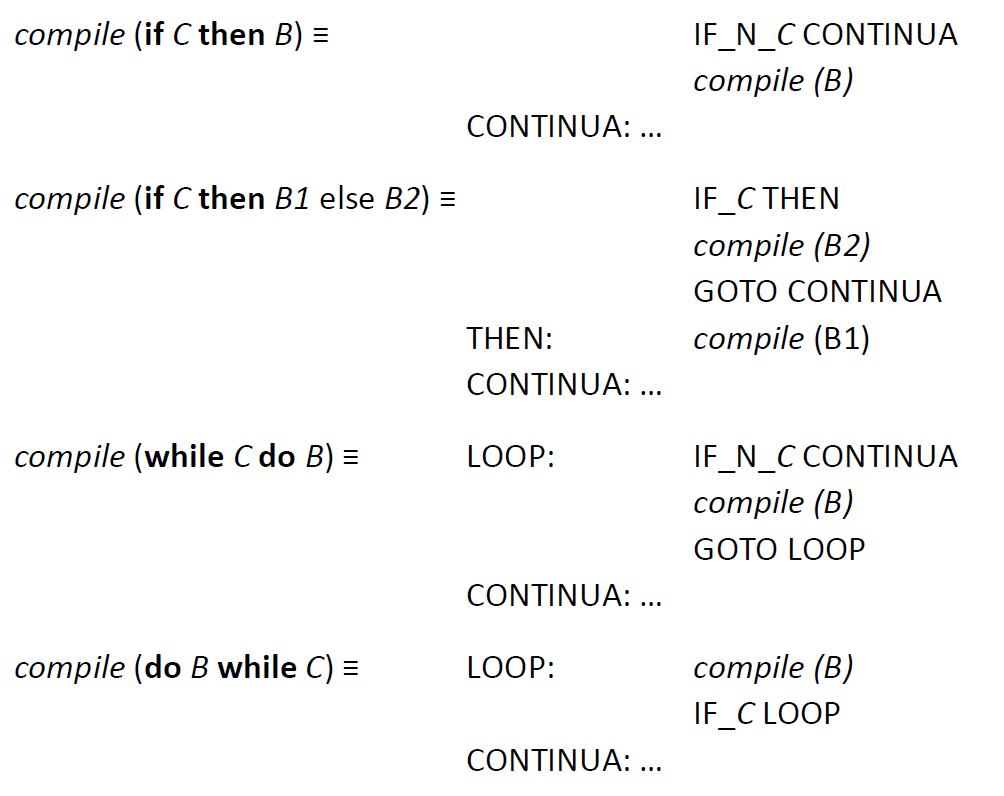
\includegraphics[width=\textwidth]{immagini/Regole.png}
\end{figure}

\subsection{Compilazioni di procedure e funzioni}

Si consideri una computazione che contenga una procedura o una funzione, nel seguito indicata con \textit{S}.

I problemi da risolvere per la sua compilazione sono essenzialmente:

\begin{enumerate}
    \item \textit{meccanismo di chiamata} a \textit{S} e \textit{di ritorno} da \textit{S} al programma chiamante;
    \item \textit{passaggio di parametri e risultati} tra programma chiamante e programma chiamato \textit{S}.
\end{enumerate}
\begin{enumerate}
    \item All'atto della \textit{chiamata}, nel programma chiamante occorre salvare l'indirizzo di ritorno ed effettuare un salto all'indirizzo di \textit{S}:\ queste due azioni sono effettuate dall'unica istruzione $\mathtt{CALL\ R_{proc}}, \mathtt{R_{ret}}$.\ Il \textit{ritorno} da \textit{S} al programma chiamante avviene semplicemente con l'istruzione (già nota) $\mathtt{GOTO\ R_{ret}}$ dove $\mathtt{R_{ret}}$ è l'indirizzo del registro nel quale è stato salvato il valore di IC+1 al momento della chiamata.
    \item \textbf{Passaggio dei parametri}:\ nel caso più semplice, ma piuttosto frequente, in cui i parametri di ingresso e di uscita di \textit{S} siano relativamente pochi, il passaggio di tali parametri può essere effettuato attraverso registri generali.\ Altrimenti, e comunque qualora le procedure/funzioni siano annidate o ricorsive, occorre utilizzare una struttura dati in memoria di tipo pila gestita mediante istruzioni di \texttt{Load} e \texttt{Store}.
\end{enumerate}

\begin{figure}[H]
    \centering
    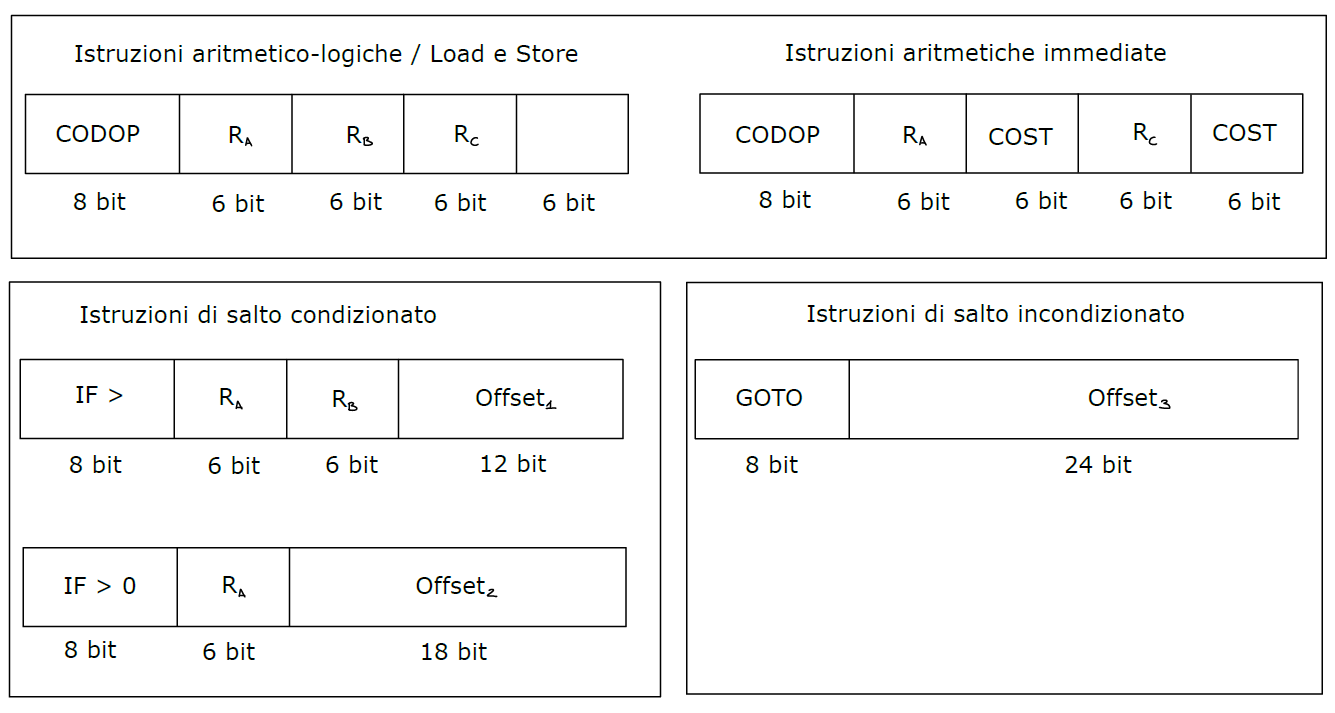
\includegraphics[width=\textwidth]{immagini/Istruzioni.png}
\end{figure}
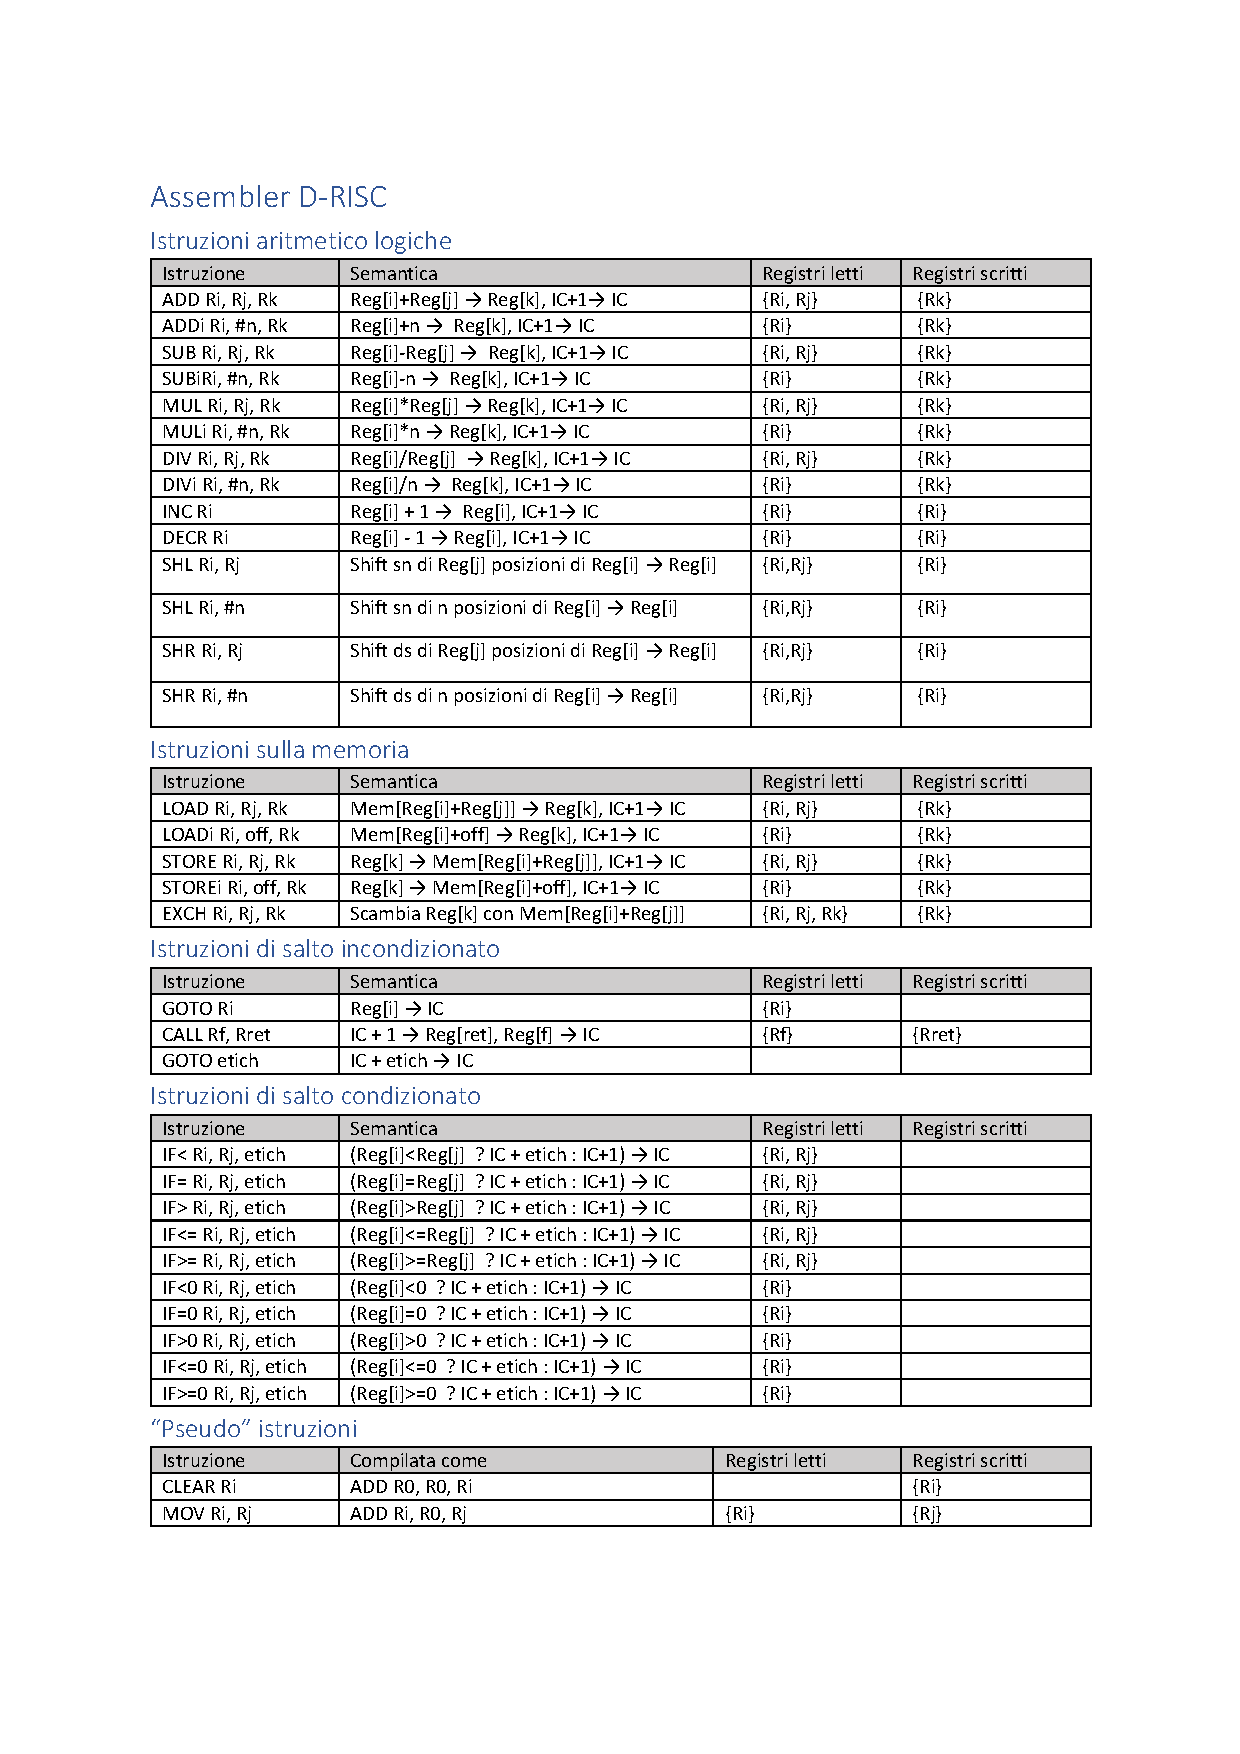
\includepdf[pages=-]{istruzioni ass DRISC}

